\documentclass[border=8pt]{standalone}
\usepackage[T1]{fontenc}\usepackage{helvet}\renewcommand{\familydefault}{\sfdefault}
\usepackage{tikz}\usetikzlibrary{arrows.meta, positioning, calc, backgrounds}
\definecolor{ink}{HTML}{1a1916}
\definecolor{inktwo}{HTML}{3a3a35}
\definecolor{inkthree}{HTML}{6a6862}
\definecolor{rule}{HTML}{b8b09a}
\definecolor{amber}{HTML}{a8730a}
\definecolor{red}{HTML}{c8261a}
\definecolor{paper}{HTML}{f0eee5}
\definecolor{slab}{HTML}{d8d4c6}
\tikzset{
  >={Stealth[length=2.2mm]},
  wire/.style={line width=0.8pt, ink},
  modwire/.style={line width=0.6pt, dashed, ink},
  tastewire/.style={line width=0.6pt, dashed, amber},
  gatewire/.style={line width=0.6pt, dotted, ink},
  block/.style={rectangle, draw=ink, line width=0.9pt, fill=slab, minimum width=3.0cm, minimum height=1.9cm, inner sep=0pt},
  perf/.style={rectangle, draw=ink, line width=0.7pt, minimum width=3.0cm, minimum height=0.7cm, inner sep=2pt, font=\footnotesize, text=ink},
  title/.style={font=\scriptsize\bfseries, text=ink, anchor=north, inner sep=2pt},
  jack/.style={circle, draw=ink, fill=paper, line width=0.5pt, minimum size=3.2pt, inner sep=0pt},
  plabel/.style={font=\tiny, text=inktwo, anchor=west, inner sep=1pt},
  olabel/.style={font=\tiny, text=inktwo, anchor=east, inner sep=1pt},
  settings/.style={font=\scriptsize, text=ink, align=left, anchor=north west, inner sep=1pt, text width=2.9cm},
}
\begin{document}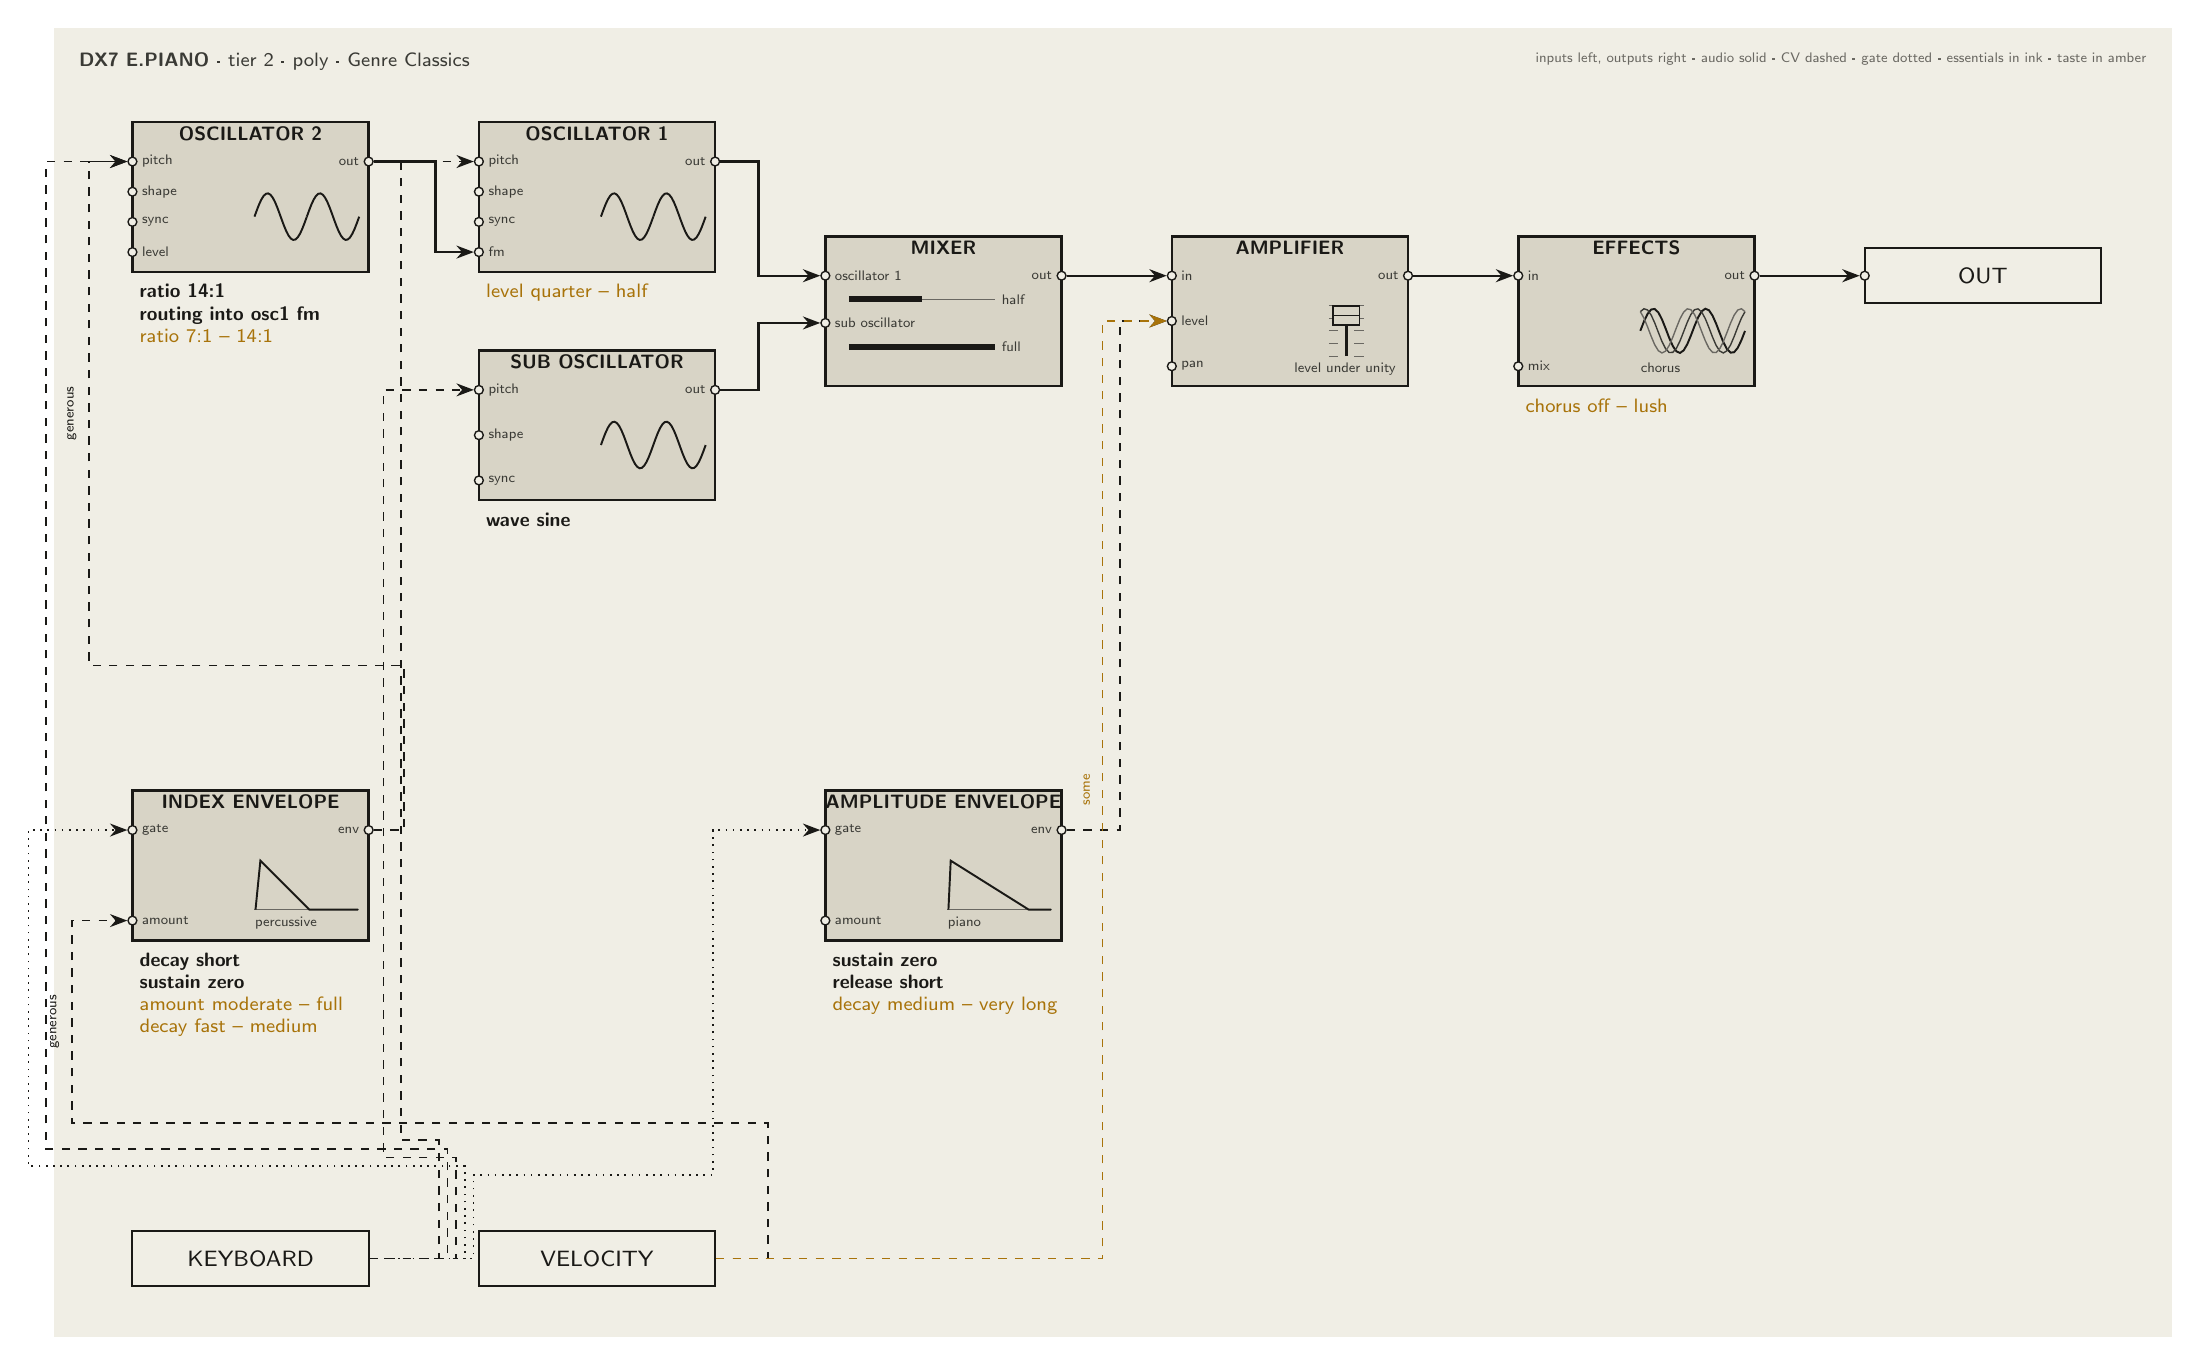
\begin{tikzpicture}
\begin{scope}[on background layer]\fill[paper] (-2.5,-13.03) rectangle (24.4,3.5999999999999996);\end{scope}
\node[block, minimum height=1.9cm] (osc1) at (4.4,1.45) {};
\node[title] at (osc1.north) {OSCILLATOR 1};
\node[jack] (osc1-pitch) at (2.9000000000000004,1.9) {};
\node[plabel] at (2.9800000000000004,1.9) {pitch};
\node[jack] (osc1-shape) at (2.9000000000000004,1.5166666666666666) {};
\node[plabel] at (2.9800000000000004,1.5166666666666666) {shape};
\node[jack] (osc1-sync) at (2.9000000000000004,1.1333333333333333) {};
\node[plabel] at (2.9800000000000004,1.1333333333333333) {sync};
\node[jack] (osc1-fm) at (2.9000000000000004,0.75) {};
\node[plabel] at (2.9800000000000004,0.75) {fm};
\node[jack] (osc1-out) at (5.9,1.9) {};
\node[olabel] at (5.82,1.9) {out};
\begin{scope}
\draw[ink, line width=0.7pt] plot[domain=0.000:0.500, samples=24, variable=\u] ({4.450+\u*1.330},{0.830+(0.740)*(0.5+0.4*sin(360*(\u*2))+0.0)});
\draw[ink, line width=0.7pt] plot[domain=0.500:1.000, samples=24, variable=\u] ({4.450+\u*1.330},{0.830+(0.740)*(0.5+0.4*sin(360*(\u*2))+0.0)});
\end{scope}
\node[settings] at (2.95,0.38) {\textcolor{amber}{level quarter -- half}};
\node[block, minimum height=1.9cm] (sub) at (4.4,-1.45) {};
\node[title] at (sub.north) {SUB OSCILLATOR};
\node[jack] (sub-pitch) at (2.9000000000000004,-1.0) {};
\node[plabel] at (2.9800000000000004,-1.0) {pitch};
\node[jack] (sub-shape) at (2.9000000000000004,-1.575) {};
\node[plabel] at (2.9800000000000004,-1.575) {shape};
\node[jack] (sub-sync) at (2.9000000000000004,-2.15) {};
\node[plabel] at (2.9800000000000004,-2.15) {sync};
\node[jack] (sub-out) at (5.9,-1.0) {};
\node[olabel] at (5.82,-1.0) {out};
\begin{scope}
\draw[ink, line width=0.7pt] plot[domain=0.000:0.500, samples=24, variable=\u] ({4.450+\u*1.330},{-2.070+(0.740)*(0.5+0.4*sin(360*(\u*2))+0.0)});
\draw[ink, line width=0.7pt] plot[domain=0.500:1.000, samples=24, variable=\u] ({4.450+\u*1.330},{-2.070+(0.740)*(0.5+0.4*sin(360*(\u*2))+0.0)});
\end{scope}
\node[settings] at (2.95,-2.52) {\textbf{wave sine}};
\node[block, minimum height=1.9cm] (osc2) at (0.0,1.45) {};
\node[title] at (osc2.north) {OSCILLATOR 2};
\node[jack] (osc2-pitch) at (-1.5,1.9) {};
\node[plabel] at (-1.42,1.9) {pitch};
\node[jack] (osc2-shape) at (-1.5,1.5166666666666666) {};
\node[plabel] at (-1.42,1.5166666666666666) {shape};
\node[jack] (osc2-sync) at (-1.5,1.1333333333333333) {};
\node[plabel] at (-1.42,1.1333333333333333) {sync};
\node[jack] (osc2-level) at (-1.5,0.75) {};
\node[plabel] at (-1.42,0.75) {level};
\node[jack] (osc2-out) at (1.5,1.9) {};
\node[olabel] at (1.42,1.9) {out};
\begin{scope}
\draw[ink, line width=0.7pt] plot[domain=0.000:0.500, samples=24, variable=\u] ({0.050+\u*1.330},{0.830+(0.740)*(0.5+0.4*sin(360*(\u*2))+0.0)});
\draw[ink, line width=0.7pt] plot[domain=0.500:1.000, samples=24, variable=\u] ({0.050+\u*1.330},{0.830+(0.740)*(0.5+0.4*sin(360*(\u*2))+0.0)});
\end{scope}
\node[settings] at (-1.45,0.38) {\textbf{ratio 14:1} \\ \textbf{routing into osc1 fm} \\ \textcolor{amber}{ratio 7:1 -- 14:1}};
\node[block, minimum height=1.9cm] (mix) at (8.8,0.0) {};
\node[title] at (mix.north) {MIXER};
\node[jack] (mix-osc1) at (7.300000000000001,0.44999999999999996) {};
\node[plabel] at (7.380000000000001,0.44999999999999996) {oscillator 1};
\draw[inkthree, line width=0.3pt] (7.600,0.150) -- (9.450,0.150);
\draw[ink, line width=2.2pt] (7.600,0.150) -- (8.525,0.150);
\node[font=\tiny, text=inktwo, anchor=west, inner sep=1pt] at (9.500,0.150) {half};
\node[jack] (mix-sub) at (7.300000000000001,-0.15000000000000002) {};
\node[plabel] at (7.380000000000001,-0.15000000000000002) {sub oscillator};
\draw[inkthree, line width=0.3pt] (7.600,-0.450) -- (9.450,-0.450);
\draw[ink, line width=2.2pt] (7.600,-0.450) -- (9.450,-0.450);
\node[font=\tiny, text=inktwo, anchor=west, inner sep=1pt] at (9.500,-0.450) {full};
\node[jack] (mix-out) at (10.3,0.44999999999999996) {};
\node[olabel] at (10.22,0.44999999999999996) {out};
\node[block, minimum height=1.9cm] (amp) at (13.200000000000001,0.0) {};
\node[title] at (amp.north) {AMPLIFIER};
\node[jack] (amp-in) at (11.700000000000001,0.44999999999999996) {};
\node[plabel] at (11.780000000000001,0.44999999999999996) {in};
\node[jack] (amp-level) at (11.700000000000001,-0.125) {};
\node[plabel] at (11.780000000000001,-0.125) {level};
\node[jack] (amp-pan) at (11.700000000000001,-0.7) {};
\node[plabel] at (11.780000000000001,-0.7) {pan};
\node[jack] (amp-out) at (14.700000000000001,0.44999999999999996) {};
\node[olabel] at (14.620000000000001,0.44999999999999996) {out};
\begin{scope}
\draw[ink, line width=1.2pt] (13.915,-0.570) -- (13.915,0.070);
\draw[inkthree, line width=0.3pt] (13.695,-0.570) -- (13.815,-0.570) (14.015,-0.570) -- (14.135,-0.570);
\draw[inkthree, line width=0.3pt] (13.695,-0.410) -- (13.815,-0.410) (14.015,-0.410) -- (14.135,-0.410);
\draw[inkthree, line width=0.3pt] (13.695,-0.250) -- (13.815,-0.250) (14.015,-0.250) -- (14.135,-0.250);
\draw[inkthree, line width=0.3pt] (13.695,-0.090) -- (13.815,-0.090) (14.015,-0.090) -- (14.135,-0.090);
\draw[inkthree, line width=0.3pt] (13.695,0.070) -- (13.815,0.070) (14.015,0.070) -- (14.135,0.070);
\fill[slab, draw=ink, line width=0.6pt] (13.745,-0.178) rectangle (14.085,0.062);
\draw[ink, line width=0.5pt] (13.745,-0.058) -- (14.085,-0.058);
\node[font=\tiny, text=inktwo, anchor=north west, inner sep=0pt] at (13.250,-0.650) {level under unity};
\end{scope}
\node[block, minimum height=1.9cm] (fx) at (17.6,0.0) {};
\node[title] at (fx.north) {EFFECTS};
\node[jack] (fx-in) at (16.1,0.44999999999999996) {};
\node[plabel] at (16.18,0.44999999999999996) {in};
\node[jack] (fx-mix) at (16.1,-0.7) {};
\node[plabel] at (16.18,-0.7) {mix};
\node[jack] (fx-out) at (19.1,0.44999999999999996) {};
\node[olabel] at (19.020000000000003,0.44999999999999996) {out};
\begin{scope}
\draw[ink, line width=0.7pt] plot[domain=0.000:1.000, samples=30, variable=\u] ({17.650+\u*1.330},{-0.620+(0.740)*(0.5+0.38*sin(360*((\u-0.000)/1.000)*2+0))});
\draw[inktwo, line width=0.5pt] plot[domain=0.000:1.000, samples=30, variable=\u] ({17.650+\u*1.330},{-0.620+(0.740)*(0.5+0.38*sin(360*((\u-0.000)/1.000)*2+60))});
\draw[inkthree, line width=0.5pt] plot[domain=0.000:1.000, samples=30, variable=\u] ({17.650+\u*1.330},{-0.620+(0.740)*(0.5+0.38*sin(360*((\u-0.000)/1.000)*2+120))});
\node[font=\tiny, text=inktwo, anchor=north west, inner sep=0pt] at (17.650,-0.650) {chorus};
\end{scope}
\node[settings] at (16.150000000000002,-1.0699999999999998) {\textcolor{amber}{chorus off -- lush}};
\node[block, minimum height=1.9cm] (menv) at (0.0,-7.04) {};
\node[title] at (menv.north) {INDEX ENVELOPE};
\node[jack] (menv-gate) at (-1.5,-6.59) {};
\node[plabel] at (-1.42,-6.59) {gate};
\node[jack] (menv-amount) at (-1.5,-7.74) {};
\node[plabel] at (-1.42,-7.74) {amount};
\node[jack] (menv-out) at (1.5,-6.59) {};
\node[olabel] at (1.42,-6.59) {env};
\begin{scope}
\draw[inkthree, line width=0.3pt] (0.050,-7.601) -- (1.380,-7.601);
\draw[ink, line width=0.7pt] (0.063,-7.601) -- (0.125,-6.979) -- (0.746,-7.601) -- (0.746,-7.601) -- (1.367,-7.601);
\node[font=\tiny, text=inktwo, anchor=north west, inner sep=0pt] at (0.050,-7.690) {percussive};
\end{scope}
\node[settings] at (-1.45,-8.11) {\textbf{decay short} \\ \textbf{sustain zero} \\ \textcolor{amber}{amount moderate -- full} \\ \textcolor{amber}{decay fast -- medium}};
\node[block, minimum height=1.9cm] (aenv) at (8.8,-7.04) {};
\node[title] at (aenv.north) {AMPLITUDE ENVELOPE};
\node[jack] (aenv-gate) at (7.300000000000001,-6.59) {};
\node[plabel] at (7.380000000000001,-6.59) {gate};
\node[jack] (aenv-amount) at (7.300000000000001,-7.74) {};
\node[plabel] at (7.380000000000001,-7.74) {amount};
\node[jack] (aenv-out) at (10.3,-6.59) {};
\node[olabel] at (10.22,-6.59) {env};
\begin{scope}
\draw[inkthree, line width=0.3pt] (8.850,-7.601) -- (10.180,-7.601);
\draw[ink, line width=0.7pt] (8.863,-7.601) -- (8.892,-6.979) -- (9.883,-7.601) -- (9.883,-7.601) -- (10.167,-7.601);
\node[font=\tiny, text=inktwo, anchor=north west, inner sep=0pt] at (8.850,-7.690) {piano};
\end{scope}
\node[settings] at (7.3500000000000005,-8.11) {\textbf{sustain zero} \\ \textbf{release short} \\ \textcolor{amber}{decay medium -- very long}};
\node[perf] (key) at (0.0,-12.03) {KEYBOARD};
\node[perf] (vel) at (4.4,-12.03) {VELOCITY};
\node[perf, fill=paper] (out) at (22.0,0.44999999999999996) {OUT}; \node[jack] (out-in) at (20.5,0.44999999999999996) {};
\draw[wire,->] (osc2-out) -- (2.3500000000000005,1.9) -- (2.3500000000000005,0.75) -- (osc1-fm);
\draw[wire,->] (osc1-out) -- (6.45,1.9) |- (mix-osc1);
\draw[wire,->] (sub-out) -- (6.45,-1.0) |- (mix-sub);
\draw[wire,->] (mix-out) -- (amp-in);
\draw[wire,->] (amp-out) -- (fx-in);
\draw[wire,->] (fx-out) -- (out-in);
\draw[modwire,->] (menv-out) -- (1.95,-6.59) -- (1.95,-4.5) -- (-2.05,-4.5) -- (-2.05,1.9) -- (osc2-pitch);
\node[font=\tiny, text=ink, anchor=south, inner sep=1pt, rotate=90] at (-2.17,-1.3) {generous};
\draw[modwire,->] (aenv-out) -- (11.040000000000001,-6.59) -- (11.040000000000001,-0.125) -- (amp-level);
\draw[modwire,->] (vel.east) -- (6.57,-12.03) -- (6.57,-10.31) -- (-2.27,-10.31) -- (-2.27,-7.74) -- (menv-amount);
\node[font=\tiny, text=ink, anchor=south, inner sep=1pt, rotate=90] at (-2.39,-9.025) {generous};
\draw[tastewire,->] (vel.east) -- (10.82,-12.03) -- (10.82,-0.125) -- (amp-level);
\node[font=\tiny, text=amber, anchor=south, inner sep=1pt, rotate=90] at (10.700000000000001,-6.0775) {some};
\draw[modwire,->] (key.east) -- (2.39,-12.03) -- (2.39,-10.53) -- (1.9100000000000006,-10.53) -- (1.9100000000000006,1.9) -- (osc1-pitch);
\draw[modwire,->] (key.east) -- (2.5,-12.03) -- (2.5,-10.64) -- (-2.5999999999999996,-10.64) -- (-2.5999999999999996,1.9) -- (osc2-pitch);
\draw[modwire,->] (key.east) -- (2.61,-12.03) -- (2.61,-10.75) -- (1.6900000000000004,-10.75) -- (1.6900000000000004,-1.0) -- (sub-pitch);
\draw[gatewire,->] (key.east) -- (2.7199999999999998,-12.03) -- (2.7199999999999998,-10.86) -- (-2.82,-10.86) -- (-2.82,-6.59) -- (menv-gate);
\draw[gatewire,->] (key.east) -- (2.83,-12.03) -- (2.83,-10.97) -- (5.870000000000001,-10.97) -- (5.870000000000001,-6.59) -- (aenv-gate);
\node[anchor=north west, font=\scriptsize, text=inktwo] at (-2.3,3.3999999999999995) {\textbf{DX7 E.PIANO} · tier 2 · poly · Genre Classics};
\node[anchor=north east, font=\tiny, text=inkthree] at (24.2,3.3999999999999995) {inputs left, outputs right · audio solid · CV dashed · gate dotted · essentials in ink · taste in amber};
\end{tikzpicture}\end{document}
